\section{Introduction}
Lot of work on arbitrary mesh
\cite{palmer_ane,palmer_proc,palmer_fe,wachspress,cell_centered_diff,mimetic}. 
Polygonal cells can potentially reduce the number of unknowns in 
our mesh, while maintaining symmetry within the mesh. We show this potential 
reduction in number of unknowns for a hexagonal cell versus the same space divided 
using triangles:
\begin{figure}[H]
\centering
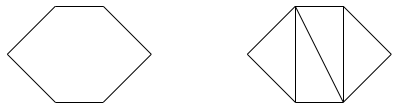
\includegraphics[width=0.5\textwidth]{hex_tri_cells}
\caption{Hexagonal cell versus triangle cells}
\end{figure}
We see that if there is one unknown per vertices, the hexagonal cell has 6
unknowns compared to the 12 unknowns of triangle cells. Polygonal cells can
also be used for adaptive mesh refinement (AMR) problems without having to
deal with hanging nodes \cite{arbitrary_hanging_nodes,dealII_hanging_nodes,
locally_hanging_nodes}. The left cell on the figure below is a pentagon whereas 
the two cells on the right are quadrilaterals:
\begin{figure}[H]
\centering
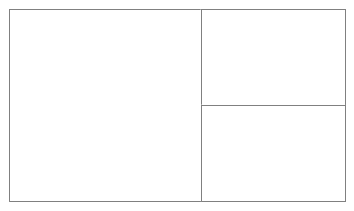
\includegraphics[width=0.3\textwidth]{amr}
\caption{AMR mesh}
\end{figure}
Using MIP requires us to solve SPD equations. This has usually been done using 
conjugate gradient preconditioned by SSOR, but in this research we will test the 
effectiveness of algebraic multigrid methods (AMG) to precondition the Krylov solver 
\cite{amg,amg_course}. Algebraic multigrid methods allow to use multigrid
techniques when there is no grid or that the mesh is unstructured. Instead of
using a succession of grids based on the geometry of the problems, the grids
are based on properties of the matrix. This allows to use AMG as black-box
solvers or preconditioners.
